\chapter{Introduction}
\label{introduction}

\begin{comment}
    introduction: motivation (why we are using batteries, due to carbon print and sustainability), problem you target and why it is a problem, then your solution, thesis outline.
\end{comment}

\section{Motivation}

\subsection*{Industry background: the EV market}

The global electric vehicle (EV) market has expanded rapidly over the past decade, driven by technological advances, supportive government policies, and increasing environmental awareness.

According to the International Energy Agency (IEA), global electric vehicle sales rose from approximately 3 million in 2020 to more than 16.6 million in 2024~\autocite{iea2024ev_sales}, representing a compound annual growth rate (CAGR) of roughly 53.4\%.

\begin{figure}[H]
    \centering
    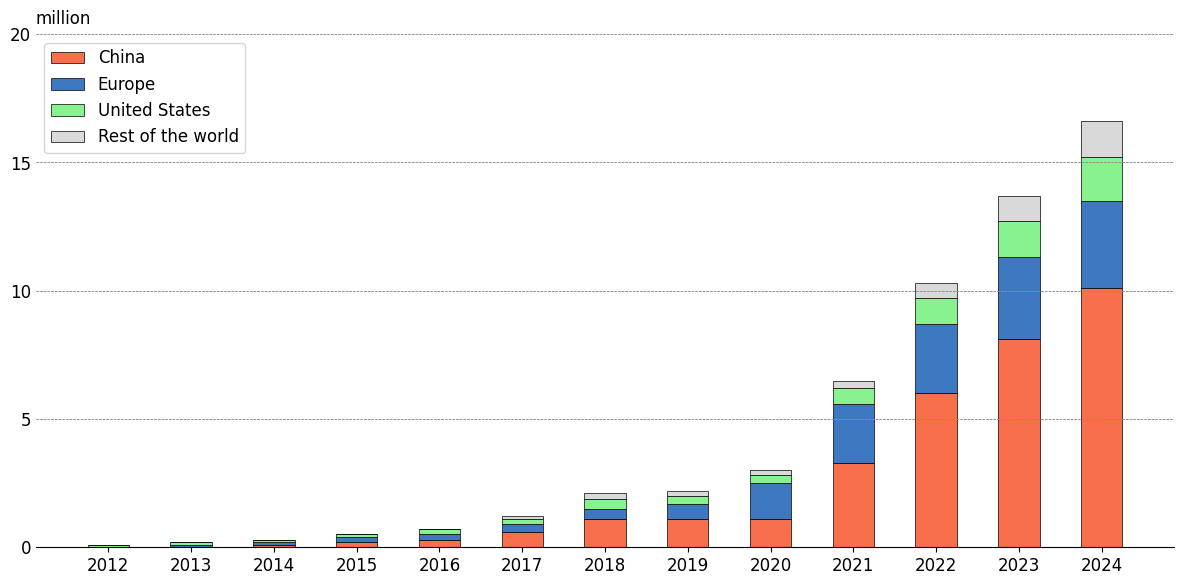
\includegraphics[width=1\linewidth]{images/ch1_EV_sales.png}
    \caption{Electric vehicle sales, 2012--2024~\autocite{iea2024ev_sales}}
    \label{fig:ev_sales}
\end{figure}

Based on current policies and trends, the rollout of electric vehicles is set to avoid the need for nearly 6 million barrels of oil per day by 2030~\autocite{iea2024ev_outlook}, significantly contributing to the reduction of fossil fuel dependence and the achievement of global carbon neutrality goals.


\subsection*{Technical foundation: why battery monitoring matters}

The battery is the single most critical component of an electric vehicle. Accurate, real-time monitoring of its internal state is therefore essential: it directly affects safety, range prediction, charging strategy, and the overall lifetime cost of the vehicle.

A Battery Management System (BMS) must track two fundamental parameters:

\begin{itemize}
    \item \textbf{State of Charge (SoC)} indicates the remaining usable energy as a fraction of the battery's current maximum capacity. It varies on short timescales (minutes to hours) and can be estimated from voltage and current measurements. SoC accuracy governs range prediction and prevents over-charge or over-discharge events.

    \item \textbf{State of Health (SoH)} quantifies the long-term degradation of the battery relative to its original condition. It is typically defined as:
    \begin{equation}
    \label{eq:soh}
    SoH = \frac{C_\text{current}}{C_\text{initial}} \times 100\%
    \end{equation}
    where $C_\text{current}$ is the present full-charge capacity and $C_\text{initial}$ is the rated capacity of a new cell. A fresh battery starts at $SoH = 100\%$; when the value drops below 70--80\%, the battery is generally considered to have reached the end of its useful automotive life.
\end{itemize}

This thesis focuses on \textbf{SoH estimation}. Unlike SoC, SoH degrades slowly — over months or years — and its trajectory is shaped by a non-linear interplay of temperature, charge/discharge rate, depth of discharge, and usage history. Moreover, SoH cannot be measured directly by a simple sensor; it must be inferred from changes in observable quantities such as capacity, internal resistance, and voltage profiles during operation.

Unreliable SoH estimates carry serious consequences. Overestimating remaining health can lead to unexpected performance drops, insufficient power delivery, or safety hazards. Underestimating it may trigger premature battery replacement, wasting economic value.

Accurate SoH estimation is therefore a foundational task in modern EV design — and not only for its own sake. SoH plays a decisive role in SoC estimation, and the relationship goes deeper than the obvious capacity scaling ($SoH \times C_\text{initial}$). As a battery ages, its internal electrochemical characteristics shift: the open-circuit voltage curve changes shape, the internal resistance increases, and the dynamic response under load is altered. In effect, \textbf{a battery at $SoH = 90\%$ and a battery at $SoH = 75\%$ behave as different systems}, and a SoC model calibrated for one aging stage will not perform well at another. An accurate, up-to-date SoH estimate is therefore the key that tells the BMS which SoC model — or which set of model parameters — to apply at any point in the battery's life. Getting SoH right is the prerequisite for a reliable BMS, and it is the problem this thesis tackles head-on.


\section{Problem Statement}

Despite decades of research, deploying a practical SoH estimation system on a production vehicle remains a multi-faceted challenge. The difficulties can be understood as a series of unresolved tensions, each layer exposing a deeper problem.

\subsection*{Layer 1 --- Model-based methods hit a computational wall}

Traditional battery modeling follows two paths. Electrochemical models, grounded in first-principles physics, describe the internal reactions, diffusion, and transport processes with high fidelity. Their accuracy, however, comes at the cost of solving coupled partial differential equations — an effort far beyond the capabilities of a real-time automotive microcontroller. Simplified variants such as the single-particle model reduce the computational burden but lose accuracy under high C-rate conditions.

Equivalent circuit models (ECMs) take the opposite trade-off: they approximate battery dynamics with resistor--capacitor networks and, when paired with filters such as the extended Kalman filter (EKF)~\autocite{ECM_EKF}, unscented Kalman filter~\autocite{ECM_UKF}, or particle filter~\autocite{ECM_PF}, can run in real time on modest hardware. This combination is the current industrial standard. Yet ECM parameters drift as the battery ages, requiring labor-intensive recalibration. Moreover, ECM accuracy degrades outside the calibrated temperature and load envelope, precisely the conditions where reliable monitoring matters most. Fundamentally, an RC network cannot capture the complex, history-dependent nonlinearities of battery aging.

\subsection*{Layer 2 --- Data-driven methods stop at simulation}

Machine learning (ML) and deep learning (DL) offer a way around the limitations of explicit physical models. Instead of hand-crafting equations, these methods learn the mapping from measurable external signals — voltage, current, temperature — to internal battery states directly from historical data. Architectures such as Long Short-Term Memory (LSTM) networks, bidirectional LSTM (BiLSTM), and convolutional neural networks have demonstrated impressive SoH estimation accuracy on public benchmarks, often reporting mean absolute errors below 2\%~\autocite{Nozarijouybari2024}.

The gap is not one of accuracy but of deployment. The overwhelming majority of ML-based SoH studies remain at the offline validation stage: models are trained and evaluated in Python on a server, and their deployment on real BMS hardware is either listed as future work or not discussed at all. The distance between a Python script and a production microcontroller is vast — it involves model conversion, memory budgeting, integration with bare-metal firmware, and validation under real-time constraints.

\subsection*{Layer 3 --- Cloud vs.\ edge: neither path is free}

A natural response to the deployment gap is to move the inference workload to a more capable platform.

Cloud-centric architectures stream battery data to remote servers, where complex models run without hardware constraints. This approach introduces unacceptable drawbacks for a safety-critical automotive function: round-trip latency on the order of hundreds of milliseconds, continuous bandwidth consumption for multi-cell high-frequency data, loss of functionality in areas without network coverage, and exposure of sensitive operational data to external infrastructure.

Edge-based architectures address these concerns by running inference directly on the vehicle's BMS microcontroller. Latency drops to microseconds, no connectivity is required, and data stays local. The trade-off is severe: an automotive MCU offers a few hundred kilobytes of RAM, a few megabytes of flash, and a CPU core running at tens to low hundreds of MHz — roughly five orders of magnitude fewer resources than the GPU server on which the model was trained.

\subsection*{Layer 4 --- The SoC--SoH coupling problem (this thesis' entry point)}

Even if an ML model is successfully deployed on an edge MCU, a longer-term system-level issue arises when we consider how SoC and SoH interact in a real BMS.

As noted in Section 1.2, SoC estimation depends on knowing the battery's true current capacity — which is $SoH \times C_\text{initial}$. When SoH degrades but the BMS continues to use a stale capacity value, SoC estimates become systematically biased, growing worse over time. In a complete BMS architecture, therefore, SoC and SoH cannot be treated in isolation: the SoC model must receive up-to-date SoH information to remain accurate.

This coupling points toward a \textbf{dual-model architecture}, originally proposed by Alamin~\autocite{Alamin2023}: a SoH model that tracks long-term degradation, and a SoC model that uses the SoH estimate as an input parameter. In this design, only the SoC model requires periodic over-the-air (OTA) updates — triggered when SoH has drifted by a meaningful amount — while the SoH model itself is built for long-term robustness and deployed once.

In the course of this thesis, the author implemented and tested this dual-model pipeline. The SoH model, based on LightGBM, was trained, compiled, and deployed on hardware (see Chapter~\ref{methodology} and Chapter~\ref{experiment}). A SoC model was also trained with SoH as an input feature. However, preliminary experiments revealed that SoH estimation errors propagated into the SoC model, amplifying the overall error. This finding motivated the decision to focus the thesis on the SoH component: until the SoH model is sufficiently accurate and robust, the dual-model pipeline cannot function as intended.

Most existing data-driven SoH approaches — including the few that have reached automotive hardware — further compound this difficulty by assuming a fixed input window length. Sammartino et al.~\autocite{Sammartino2021}, who deployed a BiLSTM on the same SPC58 MCU family used in this thesis, fix the window at 20 samples and assume every discharge cycle begins from a fully charged battery. In real-world driving, discharge events start at arbitrary SoC levels, sampling rates can differ across BMS generations, and the shape and duration of voltage and current profiles shift as the battery ages. A fixed-window model trained on laboratory data may not remain accurate in the field, and deep learning architectures such as LSTMs cannot be dynamically resized at inference time. Training a new model for changed conditions requires collecting new data, running the full pipeline on a server, and delivering the updated model via OTA — a logistically expensive process that is impractical to perform frequently at fleet scale.

These observations converge on a clear priority: \textbf{the SoH model must be both accurate enough to anchor the SoC estimator, and robust enough to handle variable input conditions without frequent retraining.} Getting SoH right is not an end in itself — it is the prerequisite for a deployable dual-model BMS.


\section{Research Aims}

This thesis operates within a broader \textbf{Digital Twin} framework proposed by Alamin~\autocite{Alamin2023}. The architecture envisions two on-board ML models working in concert: a \textbf{SoH model} that tracks long-term battery degradation, and a \textbf{SoC model} that receives the SoH estimate as an input. When the SoH estimate drifts beyond a threshold, the cloud retrains the SoC model (which depends on SoH) and delivers the update over the air (OTA). The SoH model itself is designed for deployment-time robustness and should not require frequent updates.

Within this framework, the present thesis focuses on the \textbf{SoH component} and on the design of the OTA mechanism that would serve the SoC model. The work consists of three interconnected efforts:

\begin{enumerate}
    \item \textbf{A lightweight SoH estimation model trained for input-length robustness.} A gradient-boosted decision tree ensemble (LightGBM) is trained on data segmented with multiple window lengths ($wlen \in \{20, 30, 40, 50, 60\}$). Because the model operates on a fixed-size feature vector rather than on a raw temporal sequence, a single ensemble can process windows of arbitrary length without modification. The model is compiled to C code and deployed on an automotive-grade microcontroller, delivering real-time inference without cloud dependency.

    \item \textbf{Preliminary experimentation with the dual-model pipeline.} A SoC estimation model incorporating the SoH estimate as an input feature was trained and evaluated. The experiment confirmed that SoH errors propagate into SoC predictions, reinforcing the conclusion that \textbf{SoH accuracy must be established first} before the full dual-model architecture can deliver reliable end-to-end performance. This insight defines the scope of the thesis: it concentrates on SoH as the foundational layer, while the SoC integration remains a target for future work.

    \item \textbf{An over-the-air (OTA) update mechanism (design).} The OTA mechanism is designed to support remote updates of the SoC model as the battery ages. The design covers the full update lifecycle: on-board data accumulation, cloud-side retraining triggers, secure model packaging and transmission, A/B-partition on-device installation, and a fallback to a factory-programmed golden model.
\end{enumerate}

In summary, this thesis builds the SoH foundation of a dual-model Digital Twin BMS: it develops, compiles, deploys, and validates the SoH estimator; it identifies the error-propagation challenge that must be solved before SoC can follow; and it lays out the OTA infrastructure that will eventually keep the SoC model current.


\section{Contributions}

The Digital Twin dual-model architecture underpinning this thesis was proposed by Alamin~\autocite{Alamin2023}. Within that framework, the author's contributions are as follows:

\begin{enumerate}
    \item \textbf{Multi-length segmentation and compact feature extraction.} A preprocessing strategy is developed that segments battery discharge data into windows of five different lengths and extracts a fixed ten-dimensional feature vector from each window. This enables a single model to handle arbitrary input window sizes, removing the need to train separate models for different sampling configurations.

    \item \textbf{Lightweight LightGBM-based SoH estimation model.} A gradient-boosted decision tree ensemble is trained for SoH regression, with hyperparameters optimized through Bayesian search using the Optuna framework. The resulting model balances estimation accuracy with a small memory footprint suitable for embedded deployment. On public benchmark datasets, it matches or surpasses the accuracy of a BiLSTM baseline while reducing inference latency by a factor of 11--30$\times$.

    \item \textbf{Deployment and validation on an automotive-grade MCU.} The full pipeline — feature extraction plus model inference — is deployed on the SPC58EC80E5 microcontroller by STMicroelectronics. The model is compiled to C code via the EDEN compiler (extended by collaborators to support LightGBM ensembles). Performance is evaluated along four dimensions: estimation accuracy, inference cycle count, RAM usage, and flash memory occupation. The BiLSTM baseline is reproduced on the same hardware for a fair, multi-dimensional comparison. Generalization to window lengths unseen during training is also assessed — a critical property for real-world deployment.

    \item \textbf{Design of an over-the-air update architecture.} An OTA mechanism is designed to support remote updates of the SoC model triggered by SoH degradation. The design covers the full update lifecycle: on-board data accumulation, cloud-side retraining triggers, secure model packaging and transmission, A/B-partition on-device installation, and a fallback to a factory-programmed golden model in case of failure.
\end{enumerate}


\section{Thesis Outline}

The remainder of this thesis is structured as follows.

\textbf{Chapter~\ref{background}} provides the necessary background and reviews the state of the art. It covers lithium-ion battery fundamentals and SoH degradation mechanisms, surveys SoH estimation methods (model-based and data-driven), discusses edge computing for automotive BMS and prior MCU deployment work, introduces the digital twin concept, and outlines OTA update technology.

\textbf{Chapter~\ref{methodology}} presents the proposed framework in detail, organized as a five-stage pipeline: data acquisition and preprocessing, multi-length window segmentation and feature extraction, LightGBM model training with Bayesian hyperparameter optimization, model compilation to C code via the EDEN compiler, and deployment on the SPC58EC microcontroller. The OTA update architecture is also described.

\textbf{Chapter~\ref{experiment}} reports the experimental evaluation. It describes the two public NASA battery datasets (NBD and NRD), the target hardware platform, and the evaluation metrics. Results are presented for hyperparameter configurations, SoTA comparison against BiLSTM, deployment performance across window lengths (accuracy, latency, memory), and generalization to unseen window lengths. The chapter closes with a discussion of the findings and their limitations.

\textbf{Chapter~\ref{conclusion}} concludes the thesis, summarizing the main contributions and findings, and outlines directions for future work, including hardware implementation of the OTA mechanism, validation with real-world vehicle data, model quantization, and federated learning approaches.
